\documentclass[Thesis.tex]{subfiles}
\begin{document}
\chapter{Machine Learning}
\label{chp:machine-learning}

Machine learning (ML) is a field of study concerned with building
models\footnote{The term \emph{model} is used in a very general sense, and
refers to anything that takes information as input and produces a corresponding
output.} that can perform a task without the need for explicit instructions of
how to do so. The key word is \emph{learning}; we want to enable the model to
discover the best way to solve the task at hand within the constraints that we
have imposed on it.

A simple example of a Machine Learning algorithm is linear regression, where we endeavor to
find a linear function that best fits some observed data, with respect to some
metric of what constitutes a \emph{good fit}. Other examples include
dimensionality reduction, image classification, algorithmic trading, playing
chess. Note that all of these examples \emph{could} be implemented in terms of a
large set of if-this-then-that rules, covering the explicit response to every
conceivable input. The problem with that is that we often have little to no idea
of how exactly to determine what to do for each case, not to mention the
potential infinity of rules we would need to cover all cases.

The idea of Machine Learning is to instead describe a parameterized model that
maps inputs to outputs, and a metric to quantitatively describe how good or bad
the outputs are. Then we ask the model to find the set of parameters that will
maximize the goodness (or minimize badness) of the metric. In short, Machine
Learning is saying \emph{what} you want done, rather than saying \emph{how} you
want it done.

This chapter is dedicated to presenting the relevant bits of ML that will be
relevant to the work in this thesis. As the field is vast, only a very minimal
selection of topics will be covered, and the reader is encouraged to dive deeper
into topics where interest is sparked. We start with an overview introduction of
the general process, exemplified by Linear Regression for simplicity. From there
we shall introduce Neural Networks, along with a more in depth discussion of
optimization strategies.



\section{General Procedure}

For our purposes, we will define the steps involved in developing a machine
learning model as follows:

\begin{enumerate}
  \item Define a model, $\hat f_{\hat\valpha}(\vx)$ dependent on some parameters $\hat\valpha$
  \item Define a cost function $C(\hat f_{\hat\valpha})$ - a metric of how far away from the
      ideal model $\hat f_{\hat\valpha}$ is
  \item Minimize $C(\hat f_{\hat\valpha})$ with respect to $\valpha$
\end{enumerate}

It is common to divide ML into two main sub-domains: Supervised and Unsupervised
Learning. Supervised Learning is characterized by us having access to a data set
where both inputs \emph{and} desired outputs are specified. This is possibly the
most common case, or at least the case where most \emph{want} to work with.
Examples are many, and include most regression and classification tasks.

Unsupervised Learning is (naturally) the other case, where we do not have
information about any output responses. In these cases we don't focus on
learning the output (as we have no idea of what we want that to be), but rather
on what we can learn about the inputs themselves. This can include
dimensionality reduction, clustering analysis and more.

Often we need to introduce another sub-domain for the cases that fall in
between; Reinforcement Learning. This is the domain of problems where we do not
have explicit knowledge of what outputs should be, but where we can still infer
something about whether or not an output was good. An example of this is the
problem of playing chess. While we can't label all board states with a
corresponding ``correct move'', we can say that moves that lead to
checkmate are probably good. Reinforcement learning tries to adapt a model so as
to maximize/minimize the reward/punishment that follows as a consequence of its
actions.

\gls{vmc} is a type of reinforcement learning. This is because we
do not have information about exactly what the value of the wave function should
be for every configuration, but we still have a way to evaluate the correctness
of the wave function by calculating the energy it predicts. We'll go more in
depth into how all this connects to \gls{vmc} in~\cref{sec:reinf-learning-for-vmc}.

\section{Supervised Learning}

Even though our particular interest in machine learning is for its use in \gls{vmc}, a
lot of the ideas and techniques we need come from the supervised learning
domain. Because of that, we will quickly introduce all the relevant components in the
following sections. For simplicity and clarity, we will do this through the
simplest example we have; Linear Regression.

In general for a supervised learning task, we have the following ingredients:

\begin{itemize}
\item A data set, $\mathcal{D} = \{\vx_i, \vy_i\}_{i=1}^n$, of $n$ inputs $\vx_i$
  and corresponding expected outputs $\vy_i$
\item A proposed model $\hat\vy = \hat f_{\hat\valpha}(\vx)$ that we want to
    fit to the data
\item A cost function $\mathcal{C}(\hat f_{\hat\valpha}; \mathcal{D})$ which
  to minimize with respect to the model parameters $\hat \valpha$. Note that for
  supervised learning, the cost function is dependent on the data set, allowing
  us to define metrics of how well the model reproduces the data.
\item An optimization strategy for how we should approach the minimization
\end{itemize}


\subsection{Example: Linear Regression}

\begin{figure}[h]
  \centering
  \resizebox{0.7\linewidth}{!}{%
      % This file was created by matplotlib2tikz v0.7.4.
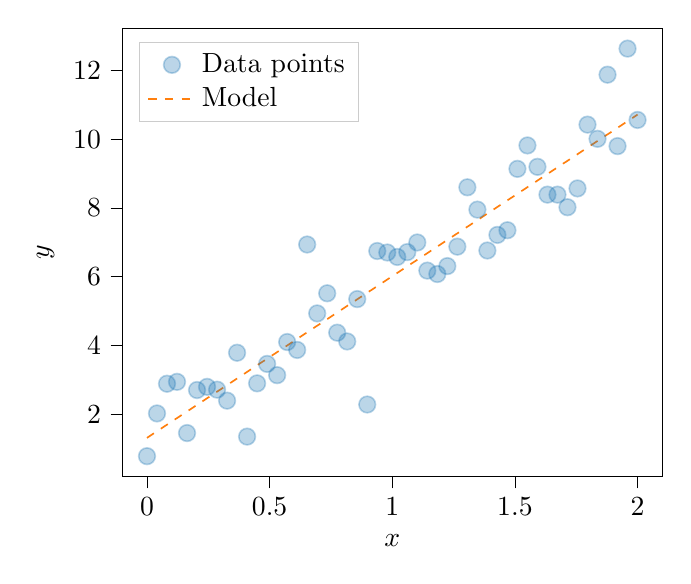
\begin{tikzpicture}

\definecolor{color0}{rgb}{0.12156862745098,0.466666666666667,0.705882352941177}
\definecolor{color1}{rgb}{1,0.498039215686275,0.0549019607843137}

\begin{axis}[
legend cell align={left},
legend style={at={(0.03,0.97)}, anchor=north west, draw=white!80.0!black},
tick align=outside,
tick pos=left,
x grid style={white!69.01960784313725!black},
xlabel={\(\displaystyle x\)},
xmin=-0.1, xmax=2.1,
xtick style={color=black},
y grid style={white!69.01960784313725!black},
ylabel={\(\displaystyle y\)},
ymin=0.189691314741281, ymax=13.2275451881467,
ytick style={color=black}
]
\addplot [semithick, color0, opacity=0.3, mark=*, mark size=3, mark options={solid}, only marks]
table {%
0 0.782321036259711
0.0408163265306122 2.02553698724508
0.0816326530612245 2.88944107434522
0.122448979591837 2.9441089401904
0.163265306122449 1.45446115861605
0.204081632653061 2.70601699452992
0.244897959183673 2.7982512222147
0.285714285714286 2.71629909502484
0.326530612244898 2.39701880091228
0.36734693877551 3.79022493810844
0.408163265306122 1.35119102451724
0.448979591836735 2.89995525231638
0.489795918367347 3.46588448890362
0.530612244897959 3.13807770245367
0.571428571428571 4.10165214881394
0.612244897959184 3.87191188228207
0.653061224489796 6.93747854025376
0.693877551020408 4.93419024396974
0.73469387755102 5.51939983211762
0.775510204081633 4.37400943826881
0.816326530612245 4.1182971232151
0.857142857142857 5.35068291521086
0.897959183673469 2.28475568552761
0.938775510204082 6.74884697743513
0.979591836734694 6.70523587752215
1.02040816326531 6.57618137004175
1.06122448979592 6.71705069578529
1.10204081632653 6.996893350413
1.14285714285714 6.17875600565952
1.18367346938776 6.07945940365117
1.22448979591837 6.31007415953039
1.26530612244898 6.87573766947214
1.30612244897959 8.60141360064448
1.3469387755102 7.95211502739419
1.38775510204082 6.76291691592648
1.42857142857143 7.21674035376784
1.46938775510204 7.35299111436777
1.51020408163265 9.1378267173966
1.55102040816327 9.81891528374901
1.59183673469388 9.19692453406167
1.63265306122449 8.38820874313926
1.6734693877551 8.38824299233666
1.71428571428571 8.02206563560459
1.75510204081633 8.5686819592157
1.79591836734694 10.4246000692698
1.83673469387755 10.0105872616746
1.87755102040816 11.8767022910241
1.91836734693878 9.79931624148078
1.95918367346939 12.6349154666283
2 10.56063787528
};
\addlegendentry{Data points}
\addplot [semithick, color1, dashed]
table {%
0 1.3144746950758
0.0408163265306122 1.50633548639334
0.0816326530612245 1.69819627771087
0.122448979591837 1.89005706902841
0.163265306122449 2.08191786034594
0.204081632653061 2.27377865166347
0.244897959183673 2.46563944298101
0.285714285714286 2.65750023429854
0.326530612244898 2.84936102561608
0.36734693877551 3.04122181693361
0.408163265306122 3.23308260825115
0.448979591836735 3.42494339956868
0.489795918367347 3.61680419088621
0.530612244897959 3.80866498220375
0.571428571428571 4.00052577352128
0.612244897959184 4.19238656483882
0.653061224489796 4.38424735615635
0.693877551020408 4.57610814747388
0.73469387755102 4.76796893879142
0.775510204081633 4.95982973010895
0.816326530612245 5.15169052142649
0.857142857142857 5.34355131274402
0.897959183673469 5.53541210406156
0.938775510204082 5.72727289537909
0.979591836734694 5.91913368669662
1.02040816326531 6.11099447801416
1.06122448979592 6.30285526933169
1.10204081632653 6.49471606064923
1.14285714285714 6.68657685196676
1.18367346938776 6.8784376432843
1.22448979591837 7.07029843460183
1.26530612244898 7.26215922591936
1.30612244897959 7.4540200172369
1.3469387755102 7.64588080855443
1.38775510204082 7.83774159987197
1.42857142857143 8.0296023911895
1.46938775510204 8.22146318250703
1.51020408163265 8.41332397382457
1.55102040816327 8.6051847651421
1.59183673469388 8.79704555645964
1.63265306122449 8.98890634777717
1.6734693877551 9.1807671390947
1.71428571428571 9.37262793041224
1.75510204081633 9.56448872172977
1.79591836734694 9.75634951304731
1.83673469387755 9.94821030436484
1.87755102040816 10.1400710956824
1.91836734693878 10.3319318869999
1.95918367346939 10.5237926783174
2 10.715653469635
};
\addlegendentry{Model}
\end{axis}

\end{tikzpicture}
  }
  \caption[Example of linear regression]{Example of linear regression applied to a simple data set of a single
    input variable. The regression tries to filter away the noise and find the
    most likely actual trend line.\citesource{writing/scripts/linear_regression_example.py}}
  \label{fig:linear-regression-example}
\end{figure}


We assume that the true underlying process, $f_{\valpha}(\vx)$, that generated
$\mathcal{D}$ is linear in the inputs $\vx$. For simplicity, we will also
assume that the outputs are scalar, $\vy \defeq y$. That is, we assume the data
was generated in the following way:
\begin{align}
  y_i = f_{\valpha}(\vx_i) + \epsilon = \vx^T\valpha + \epsilon
\end{align}
where $\valpha$ is a column vector of coefficients, and
$\epsilon\sim\mathcal{N}(0, \sigma^2)$ is normally distributed noise with zero
mean and variance $\sigma^2$, introduced via measurement inaccuracy
etc.\footnote{Note that this definition implies that $f_{\valpha}$
  has zero intercept, i.e. $f_{\valpha}(\vb{0}) = 0$. We can easily work around
  that, however, by adding a constant element to every input vector, i.e. let
  $\vx' \defeq (1\ \ \vx)$ be the new inputs. The second option is to simply
  center the data beforehand, by subtracting the mean $\overline y =
  \flatfrac{1}{n}\sum_{i=1}^n y_i$ from every $y_i$, and then optionally revert
  back whenever needed.}

\subsubsection{Model}

Based on the above assumption, we propose the following model:

\begin{align}
\hat f_{\hat\valpha}(\vx) &= \vx^T\hat\valpha.
\end{align}
Ideally we want to learn $\hat\valpha$ from the data such that
$\hat\valpha\simeq\valpha$.

\subsubsection{Cost Function}

In order to quantify which $\hat\valpha$ is optimal, we need metric to compare
by. There are several conceivable choices here, many of which might lead us to
the correct $\valpha$. Most common, at least in this case, is to use the
so-called Mean Square Error (MSE):

\begin{align}
  \mathcal{C}_\text{MSE}(\hat f_{\hat\valpha}; \mathcal{D}) &= \frac{1}{n}\sum_{i=1}^n \abs{\hat f_{\hat\valpha}(\vx_i) - y_i}^2.
\end{align}
The ``learning'' task is now expressed simply as the following optimization problem:
\begin{align}
  \label{eq:mse-optimization-problem-example}
  \hat\valpha = \argmin_{\valpha'}\,\mathcal{C}_\text{MSE}(\hat f_{\valpha'}; \mathcal{D})
\end{align}

\subsubsection{Optimization}

With data, model and cost function defined, the last step is to
solve~\cref{eq:mse-optimization-problem-example}. While this can in general be a
hard task (more on this in \cref{sec:ml-optimization}), we can
actually do this particular exercise analytically with some rather simple linear algebra. Skipping
the derivation, we get the following solution:
\begin{align}
  \hat\valpha = \qty(\vX^T\vX)^{-1}\vX\vy,
\end{align}
where $\vX = (\vx_1, \vx_2\,\dots\vx_n)^T$ is the matrix with inputs laid out in
rows, and $\vy$ is the column vector of all outputs.

\subsubsection{Regularization}

Often times it turns out to be useful to add an extra term to the cost function
that depends on the size of the parameters $\hat\valpha$. This typically takes
the following form:

\begin{align}
  \mathcal{C}(\hat f_{\hat\valpha};\mathcal{D}) &=   \mathcal{C}_\text{MSE}(\hat f_{\hat\valpha};\mathcal{D}) + \gamma\norm{\hat\valpha}_p^p,
\end{align}
where $\norm{\cdot}_p$ is the $L^p$ norm, and $\gamma$ is a parameter
we set to control the degree of regularization (typically $\gamma\ll 1$). Most
used are $p=1$ (called the LASSO loss) and $p=2$ (called the Ridge loss).

The motivation for why we might want to do this is as follows: Imagine we have
data set with $\vx_i = (x_i, 2x_i)$, that is to say we have two variables per
data point, but the two variables are directly correlated. Lastly, assume that
$y_i = 3x_i$ is the underlying function. Without any regularization, all of the
following models are equally good:

\begin{align}
  \hat\valpha^{(1)} = (3, 0),\ \hat\valpha^{(2)} = (1, 1),\ \hat\valpha^{(3)} = (-997, 500)
\end{align}
The problem is that without regularization, this particular
optimization problem ill-formed, and does not have a unique solution. While all
of the above give perfect reconstruction of the data, solutions like
$\valpha^{(3)}$ yield strange interpretations. According to this model, the
output is strongly negatively correlated with $x_1$, in complete contradiction
with the underlying truth.

While this particular example is very contrived, the point should be clear: In
some cases, depending on both the data and what model we choose, the model might
be too flexible for the task at hand. This is generally referred to as the
problem of \emph{overfitting}, and can lead to strange behavior. The opposite
problem called \emph{underfitting} refers to the case where the model is too
constrained, e.g. trying to fit a first order polynomial to
quadratic data.



\section{Gradient Based Optimization}
\label{sec:ml-optimization}

Most supervised learning tasks rely on a gradient based optimization strategy,
with the umbrella name \emph{Gradient Decent} (GD).
These methods can be summarized as follows: We want to find $\vx^*$ such that\footnote{For maximization, simply minimize $-f(\vx)$. }

\begin{align}
  \vx^* = \argmin_{\vx} g(\vx),
\end{align}
for some function $g$ that should be minimized.
We solve this by starting at some initial guess $\vx^{(0)}$ and improve it by
iterating the following recurrence relation:

\begin{align}
  \label{eq:gradient-decent-definition}
  \vx^{(n+1)} &= \vx^{(n)} + \Delta \vx^{(n)} \\
  \Delta\vx^{(n)} &= -\eta \grad{g}(\vx^{(n)})
\end{align}
where $\eta$ is a suitably chosen number, typically $\eta \ll 1$. In the
limit $n\to\infty$ (if $\eta$ is small enough), this will converge to a minimum
for $g$.

When $g=\mathcal{C}(\hat f_{\hat\valpha}; \mathcal{D})$ we have some choice in
exactly how we should compute $\grad{\mathcal{C}}$. We could compute the cost
for the entire data set, or just a single data point. These
two options are referred to as Gradient Decent (GD) and Stochastic Gradient
Decent (SGD), respectively. The latter is most often used because it is less
computationally expensive for large data sets.

Lastly we have various ways of extending the basic algorithm in
\cref{eq:gradient-decent-definition}, with more sophisticated ways of
determining $\Delta \vx^{(n)}$, some of which we will mention here.

\subsection{Fixed Learning Rate}

This is the version presented in \cref{eq:gradient-decent-definition}, in where
$\eta$ is chosen in advance and remains fixed throughout all iterations:
\begin{align}
  \label{eq:fixed-learning-rate-update-rule}
  \Delta \vx^{(n)} = -\eta \grad{g(\vx^{n})}.
\end{align}

\begin{itemize}
\item Pros:
  \begin{itemize}
    \item Easy to implement
    \item Intuitive and easy to adapt based on results
  \end{itemize}
\item Cons:
  \begin{itemize}
    \item If $\eta$ is to large it can lead to divergence or inaccurate results
    \item If $\eta$ is to small we have a higher chance of getting stuck in small, local minima.
    \item If $\eta$ is small we will need many iterations before convergence
    \item All elements of $\vx$ get the same $\eta$, even though the gradient
        elements can have significantly different magnitude and/or stability.
  \end{itemize}
\end{itemize}

\subsection{Momentum}

Two common problems arise when using the update rule
in~\cref{eq:fixed-learning-rate-update-rule}, namely that we tend to get stuck
in local minima and that unstable gradients can throw us off the right track.
The idea of momentum, first introduced by \textcite{Rumelhart-1986}, aims to
combat this by letting the update be a linear combination of the previous step
and the current one:

\begin{align}
  \label{eq:momentum-update-rule-def}
  \Delta\vx^{(n)} &= \alpha \Delta \vx^{(n-1)} - \eta \grad{g(\vx^{(n)})}.
\end{align}
This introduces another hyper-parameter $\alpha$, which again should be set to
an appropriate value. Letting $\alpha=0$
recovers~\cref{eq:fixed-learning-rate-update-rule}, and increasing values
increases the update terms' inertia.

\subsection{Individual Learning Rates per Element}

The magnitude and/or stability of the elements of $\grad{g}$ can be
significantly different from each other. A optimal single learning rate $\eta$ might
therefore not be optimal for an single element, but rather the best compromise
available. A simple fix to this is to use a separate learning rate for each
dimension:

\begin{align}
  \Delta\vx^{(n)} = -\vb{\eta}\circ\grad{g}(\vx^{(n)})
\end{align}
where $\circ$ denotes the Hadamard product (element-wise multiplication). This
allows us more flexibility and will improve results, while the obvious downside
is the increased need for hyper-parameter tuning.


\subsection{Averaging}

Another idea useful to overcome unstable gradients or poorly converging updates
is that of \emph{averaging}, invented by \textcite{Polyak-1992}. We keep the
simple update rule from~\cref{eq:fixed-learning-rate-update-rule}, but the final
$\vx^*$ we use is set to the average of all the intermediate steps:

\begin{align}
  \label{eq:averaging-update-rule-def}
  \vx^* = \frac{1}{n}\sum_{i=0}^{n-1} \vx^{(i)}.
\end{align}

\subsection{ADAM: Adaptive Moment Estimation}
\label{sec:adam}

Among the state-of-the-art algorithms available, employing both momentum,
averaging and several other ideas, is the ADAM algorithm, invented by
\textcite{KingmaB14}. It is slightly more involved, and the reader is encouraged
to read the aforementioned paper for an excellent presentation. The short story
has the algorithm defined as follows\footnote{All operations on vectors are
  element-wise. Exponentiation is expressed by superscripts \emph{not}
  surrounded in parenthesis.}:

\begin{align}
  \vb {m}^{(n+1)} &= \beta_1 \vb {m}^{(n)} + (1 - \beta_1)\grad{g(\vx^{(n)})}\\
  \vb {v}^{(n+1)} &= \beta_2 \vb {v}^{(n)} + (1 - \beta_2)\grad{g(\vx^{(n)})}\circ\grad{g(\vx^{(n)})}\\
  \vb{\hat m} &= \frac{\vb{m}^{(n+1)}}{1 - \beta_1^{n+1}}\\
  \vb{\hat v} &= \frac{\vb{v}^{(n+1)}}{1 - \beta_2^{n+1}}\\
  \Delta \vx^{(n)}&= -\eta\, \vb {\hat m}\oslash\sqrt{\vb {\hat v} + \epsilon},
  % \label{eq:adam-update-rule-def}
\end{align}
where $\eta$ is as before, $\beta_1$ and $\beta_2$ are decay rates for moment
estimates, and $\epsilon$ is a small number used to avoid division by zero
issues ($\oslash$ denotes Hadamard division, element-wise division). \textcite{KingmaB14} provide default values for all the parameters, and
in many cases these work excellently right out of the box.
\begin{align}
  \label{eq:adam-default-parameters}
  \begin{split}
    \eta &= 0.001\\
    \epsilon &= 10^{-8}
  \end{split}
  \begin{split}
    \beta_1 &= 0.9\\
    \beta_2 &= 0.999
  \end{split}
\end{align}

Especially important for us is how ADAM adapts \emph{individual} learning rates
per parameter. After all, given tens of thousands of parameters, what are the
chances that all of them have the same optimal learning rate? ADAM allows us to
account for different degrees of variability in the parameters.

We will make extensive use of ADAM in our \gls{vmc} calculations, and as we will later
see in \cref{prt:results}, it will prove to outperform vanilla SGD in all cases.

\section{Reinforcement Learning for \gls{vmc}}
\label{sec:reinf-learning-for-vmc}

As mentioned, \gls{vmc} is a type of reinforcement learning problem. While we don't
have access to a data set of configurations and their corresponding wave
function amplitude, we can say something about the goodness of any particular
wave function by measuring the expected ground state energy.

While reinforcement learning typically differs quite a lot from supervised
learning in both model type, optimization strategy etc., they are not so by
definition. When considering \gls{vmc} in particular, we can treat it exactly the same
as we would a supervised problem, with one major difference: The cost function
is \emph{not} dependent on a data set. We use the same types of models, and the
same strategies to minimize the cost function.

With this key change comes some differences. In particular, in some sense it
is impossible to overfit a model. Overfitting happens when a model performs
significantly better on the training data compared to data it has not seen
before. We detect overfitting in supervised learning by withholding some of
the training data and then evaluate the performance on this test data. This
measures the models ability to generalize information, as opposed to memorizing
exact values from the training data.

For reinforcement learning, however, what would the equivalent be? There is no
data to withhold. If a \gls{vmc} calculation suddenly results in an amazingly accurate
result, then we simply have an amazingly accurate wave function. With this in
mind, why not use an incredibly complex model? To some extent, this is the exact
argument of this thesis, and we will use some highly complex models later on.
There is, however, two limiting issues with this approach. First of is the
computational cost, which limits what we can feasibly do. Second, and more
importantly, learning becomes harder with more complex models. Just because the
model is theoretically capable of representing the wave function to great
accuracy, it does not mean that we will ever be able to learn the correct
parameters. With increasing complexity we increase the number of local
minima in the parameter space. In here lies the challenge, attempting balance
the \emph{exploration} of all possible parameter configurations with \emph{exploitation} of
promising minima.


\section{Artificial Neural Networks}
\label{sec:artificial-neural-networks}

Artificial Neural Networks (ANN, or just NN) are a broad category of
computational models, a representation of some general function $f:
\mathbb{R}^m\to\mathbb{R}^n$.\footnote{While there is nothing inherent about
  ANNs that limit us to only real values, we will not use
  complex valued networks in this work and therefore skip to mental burden of
  thinking about the complex numbers.} Their name and origin stems from an attempt to
model how neurons in animal brains react to inputs, and how they adapt to learn
new skills. As animals are quite effective at learning based on the inputs from
their surroundings, it seemed promising to emulate this
process when attempting to teach a computer new tricks. ANNs have since been the
target of extensive research, and has branched out in numerous variations that
have little to no analog in animal brains.

While the original idea to use ANNs first appeared around the middle of the 20th
century, they where initially limited, in large part due to the lacking
computational capacity of that time, and saw little use for a long time. As
computing power increased exponentially, most state-of-the-art
machine learning models today are some variation on a neural network. This
includes tasks such as natural language processing~\cite{bert-2018}, image classification and
segmentation~\cite{gpipe-2018}, and playing games such as Go~\cite{deepmind-alpha-go-zero},
Chess~\cite{deepmind-alpha-zero} and Starcraft II~\cite{vinyals_babuschkin_chung_mathieu_2019}.

The following sections are devoted to presenting the type of artificial neural
networks that we will employ in this work, including mathematical underpinnings,
architecture choices and training strategies.

\subsection{Nodes and Connections}

\begin{figure}[h]
  \centering
  \def\layersep{2.5cm}
\begin{tikzpicture}[shorten >=1pt,->,draw=black!50, node distance=\layersep]
  \tikzstyle{every pin edge}=[<-,shorten <=1pt]
  \tikzstyle{neuron}=[circle,fill=black!25,minimum size=17pt,inner sep=0pt]
  \tikzstyle{input neuron}=[neuron, fill={rgb:red,0.12156862745098;green,0.466666666666667;blue,0.705882352941177}];
  \tikzstyle{output neuron}=[neuron, fill={rgb:red,1;green,0.498039215686275;blue,0.0549019607843137}];
  \tikzstyle{hidden neuron}=[neuron, fill={rgb:red,0.172549019607843;green,0.627450980392157;blue,0.172549019607843}];
  \tikzstyle{bias neuron}=[neuron, fill={rgb:red,0.580392156862745;green,0.403921568627451;blue,0.741176470588235}];
  \tikzstyle{annot} = [text width=4em, text centered]

  % Draw the input layer nodes
  \foreach \name / \y in {1,...,4}
  % This is the same as writing \foreach \name / \y in {1/1,2/2,3/3,4/4}
  \node[input neuron, pin=left:$x_\y$] (I-\name) at (0,-\y) {};

  \node[bias neuron, pin=left:$b^{(0)}$] (I-5) at (0, -5) {};

  % Draw the hidden layer nodes
  \foreach \name / \y in {1,...,5}
  \path[yshift=0.5cm]
  node[hidden neuron] (H-\name) at (\layersep,-\y cm) {};

  \path[yshift=0.5cm] node[bias neuron, pin=left:$b^{(1)}$] (H-6) at (\layersep,-6 cm) {};

  % Draw the output layer node
  \node[output neuron,pin={[pin edge={->}]right:Output}, right of=H-3] (O) {};

  % Connect every node in the input layer with every node in the
  % hidden layer.
  \foreach \source in {1,...,5}
  \foreach \dest in {1,...,5}
  \path (I-\source) edge (H-\dest);

  % Connect every node in the hidden layer with the output layer
  \foreach \source in {1,...,6}
  \path (H-\source) edge (O);

  % Annotate the layers
  \node[annot,above of=H-1, node distance=1cm] (hl) {Hidden layer};
  \node[annot,left of=hl] {Input layer};
  \node[annot,right of=hl] {Output layer};
\end{tikzpicture}
  \caption[Illustration of an artificial neural network]{Illustration of a general Feed-Forward Neural Network architecture,
    here shown with four inputs nodes, one hidden layer of 5 nodes and a
    single output node.\citesource{writing/illustrations/neural-network.tex}}
  \label{fig:neural-network-example-diagram}
\end{figure}

First things first; What is a neural network? A neural
network\footnote{Specifically feed forward neural networks. There are some types
of exotic networks that does not fit well into this description, but they are
beyond the scope of this discussion.} is a way to express a certain type of
complex computation. We model a computation as a sequence of \emph{layers}, with
each layer consisting of \emph{nodes}, and some connections between the nodes in
each layer. By convention, we call the first layer the \emph{input} layer, the
last layer is called the \emph{output} layer, and layers in between are
generally referred to as \emph{hidden} layers.
\cref{fig:neural-network-example-diagram} shows a graphical depiction of this
general structure, exemplified for a certain number of layers/nodes.

Each node can hold a scalar value, and this value is propagated forward thorough
the connections. Each connection has an associated weight (scalar) which is
multiplied to the node's value before it is passed along. Nodes with multiple
incoming connections take the sum as its value. Finally we might also include
bias nodes, which are nodes with a fixed value. These serve the same role as the
intercept in a linear model, and enable us to - well, bias the output in some
direction. If we initialize the input layer with some values, we can think of
the network as a computation flow graph - visually representing the way
information is manipulated as it moves towards a final output.

\subsubsection{Definition}
\label{sec:ml-ann-forward-def}

 Let $a_i^{l}$ be the value of the $i$'th node in the $l$'th layer, with
$a_i^{(0)}=x_i$ being the inputs to the network. Each layer $l$ in the network
consists of a weight matrix $\mat W^{(l)}$, such that $W_{ij}^{l}$ is the
connection between $a_i^{(l-1)}$ and $a_j^{(l)}$. We also have a set of biases
$b_i^{(l)}$\footnote{In~\cref{fig:neural-network-example-diagram} the bias is
illustrated as a single node with multiple connections, while in the
mathematical notation we express the bias as a vector of values. These two are
equivalent, and the figure is drawn as is for clarity. In all equations and
code, bias is represented by as vector.}for each $a_i^{(l)}$, and finally a set
of activation functions $\sigma^{(l)}: \mathbb{R}\to\mathbb{R}$ (to be
explained). All this comes together to define the network output $f(\vx)$ as
follows:\footnote{Repeated indices within a term imply a summation. Note however
that this is not implied for superscripts. That is, $A_{ij}^{(l)}B_{jk}^{(l)}
\defeq \sum_{j} A_{ij}^{(l)}B_{jk}^{(l)}$}\footnote{While the example diagram
only has a single output, there is nothing stopping us from having
multidimensional outputs.}


 \begin{align}
   f(\vx) &= \vb{a}^{(L)}\\
   a_k^{(l)} &= \sigma^{(l)}(z_k^{(l)})\\
   z_k^{(l)} &= W^{(l)}_{ki}a_i^{(l-1)} + b^{(l)}_k
 \end{align}
This recursively defined result is calculated by starting at $l=0$ with
$\vb{a}^{(0)}\defeq \vx$ and calculating $\vb{a}^{(l+1)}$ iteratively. The
process of doing this is sometimes referred to as a \emph{forward propagation}.


\subsection{Activation Functions}
\label{sec:ml-activation-functions}

Say we set all $\sigma^{(l)}$ to the identity transformation (i.e. no
transformation). Then the above definition would be reduced to the following:

\begin{align}
  f(\vx) = \vb{z}^{(L)}\qq{with}
   z_k^{(l)} &= W^{(l)}_{ki}z_i^{(l-1)} + b^{(l)}_k
\end{align}
If you have had your morning coffee you might already see the issue here. This
is simply a series of affine transformations, and as such could be replaced with
one single, compound transformation: $\vb{z}^{L} = \mat{W}\vx + \vb{b}$. Turns
out, without an activation function, no matter how many layers we place in
between the input and output, we have just defined a convoluted way of
performing a simple affine transformation.

That is why we pump the value of each
node through a \emph{non-linear} function, $\sigma^{(l)}: \mathbb{R}\to\mathbb{R}$.
The functions $\sigma^{(l)}$ can really be any function we choose, and what to
pick largely depends on what computation we are trying to model. Some often used
options, with varying input/output domains, are listed in
\cref{tab:activation-functions-table}, and their plots are shown in
\cref{fig:activation-function-gallery}.

\subsubsection{Which Activation Functions to Choose}

While there is a great deal to possible discuss about the pros and cons of various
activation functions, a deep dive into this is beyond the scope of this
thesis. In practice, choosing an activation function comes down to trial
and error. Much of the neural network theory we have today is really more a set
of best practices and experiences documented by others. Seldom do we have a
rigorous backing for the choices we make, and most often a simple ``this worked
best'' is as good as we get.\footnote{This might be slight exaggeration in some
cases. But consider the state-of-the-art, massive networks of today -
understanding every aspect of their behavior seems a daunting, if at all
possible task. Sometimes the reasonable thing is simply to make some guesses and
see what happens.}

That said there are some things we \emph{can} consider, especially for the
output layer. If we want to interpret the output as a probability, something
like the Sigmoid function could be useful because it outputs numbers in $[0,
1]$. Similarly, if we want to do regression, perhaps the output layer should
have the identity function (i.e. no activation) so that the full spectrum
$(-\infty, \infty)$ is possible. Finally, in our case, wave functions tend to
involve exponentials and so we shall make heavy use of the exponential function
as the output transformation on our networks.

\begin{figure}[h]
  \centering
  \begin{tabular}{r|l}
  \begin{tikzpicture}[baseline,trim axis left]
    \begin{axis}[every axis plot post/.append style={
        mark=none,domain=-5:5,samples=50,smooth}, % All plots: from -2:2, 50 samples, smooth, no marks
      axis x line=bottom, % no box around the plot, only x and y axis
      axis y line=left,
      enlarge y limits=true,
      title={Sigmoid},
      width=0.4\textwidth,
      ]
      \addplot[semithick, color0] {1/(1 + exp(-x))};
      \addplot[dashed] {0.5};
    \end{axis}
  \end{tikzpicture}

  &

  \begin{tikzpicture}[baseline,trim axis right]
    \begin{axis}[every axis plot post/.append style={
        mark=none,domain=-5:5,samples=50,smooth}, % All plots: from -2:2, 50 samples, smooth, no marks
      axis x line=bottom, % no box around the plot, only x and y axis
      axis y line=right,
      enlarge y limits=true,
      title={Hyperbolic Tangent},
      width=0.4\textwidth,
      ]
      \addplot[semithick, color1] {tanh(x)};
      \addplot[dashed] {0};
    \end{axis}
  \end{tikzpicture}\\

  \begin{tikzpicture}[baseline,trim axis left]
    \begin{axis}[every axis plot post/.append style={
        mark=none,domain=-3:1.2,samples=50,smooth}, % All plots: from -2:2, 50 samples, smooth, no marks
      axis x line=bottom, % no box around the plot, only x and y axis
      axis y line=left,
      enlarge y limits=true,
      title={Exponential},
      width=0.4\textwidth,
      ]
      \addplot[semithick, color2] {exp(x)};
      \addplot[dashed] {0};
    \end{axis}
  \end{tikzpicture}

  &

  \begin{tikzpicture}[baseline,trim axis right]
    \begin{axis}[every axis plot post/.append style={
        mark=none,domain=-1:1,samples=3,}, % All plots: from -2:2, 50 samples, smooth, no marks
      axis x line=bottom, % no box around the plot, only x and y axis
      axis y line=right,
      enlarge y limits=true,
      title={ReLU},
      width=0.4\textwidth,
      ]
      \addplot[semithick, color3] {
              ifthenelse(
                  x<0,        % if
                  0,        % then
                  x           % else
              )
      };
    \end{axis}
  \end{tikzpicture}\\

  \begin{tikzpicture}[baseline,trim axis left]
    \begin{axis}[every axis plot post/.append style={
        mark=none,domain=-1:1,samples=3,}, % All plots: from -2:2, 50 samples, smooth, no marks
      axis x line=bottom, % no box around the plot, only x and y axis
      axis y line=left,
      enlarge y limits=true,
      title={Leaky ReLU},
      width=0.4\textwidth,
      ]
      \addplot[semithick, color5] {
              ifthenelse(
                  x<0,        % if
                  0.1 * x,   % then
                  x           % else
              )
      };
      \addplot[dashed] {0};
    \end{axis}
  \end{tikzpicture}
    &
  \begin{tikzpicture}[baseline,trim axis right]
    \begin{axis}[every axis plot post/.append style={
        mark=none,domain=-2:1,samples=101,smooth}, % All plots: from -2:2, 50 samples, smooth, no marks
      axis x line=bottom, % no box around the plot, only x and y axis
      axis y line=right,
      enlarge y limits=true,
      title={ELU},
      width=0.4\textwidth,
      ]
      \addplot[semithick, color4] {
              ifthenelse(
                  x<0,        % if
                  0.1*(exp(x) - 1),   % then
                  x           % else
              )
      };
      \addplot[dashed] {0};
    \end{axis}
  \end{tikzpicture}
\end{tabular}
  \caption[Gallery of selected activation functions]{Selection of activation functions, with their plots. See
    \cref{tab:activation-functions-table} for their definitions. Note that the
    plots for LReLU and EReLU involve a parameter which has been arbitrarily set
    to 0.1 in the plots, and that the actual behavior of the function might be
    different for other choices.\citesource{writing/illustrations/activation.tex}
  }
  \label{fig:activation-function-gallery}
\end{figure}

\begin{table}
  \caption[Selection of activation functions]{Selection of activation functions. See
    \cref{fig:activation-function-gallery} for the corresponding plots.}
  \label{tab:activation-functions-table}
  \begin{tabular}{ll}
    $\,$&\\
    Activation Function & Definition\\
    \hline\\
    Sigmoid & $\sigma(x) = \frac{1}{1 + \exp(-x)}$\\
    Hyperbolic Tangent & \(\sigma(x) = \tanh(x) = \frac{e^{x} - e^{-x}}{e^{x} + e^{-x}}\)\\
    Exponential & \(\sigma(x) = \exp(x)\)\\
    \textbf{Re}ctified \textbf{L}inear \textbf{U}nit (ReLU) & \(\sigma(x) = \max(0, x)\)\\
    \textbf{L}eaky ReLU (LReLU) & \(\sigma(x) = \max(ax, x)\qq{where} 0 < a < 1\)\\
    \textbf{E}xponential \textbf{L}inear \textbf{U}nit (ELU) & \(\sigma(x) = \begin{cases}x &\qq{where} x \geq 0\\ a\qty(\exp(x) - 1) &\qotherwise\end{cases}\)
  \end{tabular}
\end{table}


\subsection{Computational Flexibility}

Part of the reason why neural networks are such a great tool is their
flexibility. By simply changing the design of the network, or changing the type
of activation function in a layer, we can adapt and change the model as we need.
Even two identical networks can be tuned to model completely different data.
Neural networks merely define a loose framework for how layers and nodes come
together, and free us up to experiment.

The expressiveness of neural networks turns out to be just about as powerful as
anything could be. That is because \emph{any} (reasonable) function can be
arbitrarily well approximated by a neural network with a single hidden
layer~\cite{Cybenko-1989}. With just a single hidden layer it turns out we might
need exponentially many nodes, but if allowed to be deeper (more layers), we can
have reasonable number of nodes as well and still achieve arbitrarily good
results~\cite{Hanin-2017}. This result is known as the Universal Approximation
Theorem~\cite{Cybenko-1989, Hanin-2017}. A formal description for this is not
reproduced here, as to main point is to stress the expressive power of
neural networks.


\subsection{Backpropagation}
\label{sec:ml-backprop}

Now suitably enthusiastic about the power of neural networks, we must put our
feet back on the ground for a bit and do some working out. After all, defining a
complex model does not help us much if we cannot efficiently train it. With all
these layers and connections, a legitimate concerns is how we can determine how
to optimize the weights and biases involved.

We will be employing the Gradient Decent strategy from \cref{sec:ml-optimization},
which requires us to compute the gradient of a cost function,
$\grad_{\valpha}\mathcal{C}(f(\vx))$, w.r.t. all model parameters $\valpha$. In
our case, the parameters are all the weights, $\mat{W}^{(l)}$, and biases $\vb{b}^{(l)}$.

While the following derivation might appear to have a daunting amount of indices
and partial derivatives, it is really just a chain rule bonanza, applying the
same trick over and over until the problem gives up and yields a neat
solution.

Starting with the derivatives for the biases of the final layer:\footnote{For
  clarity: Repeated indices within a factor (still) imply a sum over said
  indices, but this is \emph{not} implied for superscripts in parenthesis.}

\begin{align}
  \pdv{\mathcal{C}}{b_k^{(L)}} &=
\pdv{\mathcal{C}}{z_i^{(L)}}\pdv{z_i^{(L)}}{b_k^{(L)}}
=\pdv{\mathcal{C}}{z_i^{(L)}}\pdv{}{b_k^{(L)}}\qty(W_{ij}^{(L)}a_j^{(L-1)} +
b_i^{(L)}) = \pdv{\mathcal{C}}{z_k^{(L)}}\defeq \delta_k^{(L)}
\end{align}
where
\begin{align}
  \delta_k^{(L)}\defeq \pdv{\mathcal{C}}{z_k^{(L)}} =
\pdv{\mathcal{C}}{a^{(L)}_{i}}\pdv{a_i^{(L)}}{z_k^{(L)}} =
\pdv{\mathcal{C}}{a^{(L)}_{i}}\pdv{\sigma^{(L)}(z_i^{(L)})}{z_k^{(L)}} =
\pdv{\mathcal{C}}{a^{(L)}_{k}}\dot\sigma^{(L)}(z_k^{(L)}).
\end{align}
This last expression we can calculate easily as the product of the derivative of
the cost function w.r.t. the network output (which should be doable for any
sensible cost function), and the derivative of the output layer activation
function evaluated at $z_k^{(L)}$ (which again is easy for any reasonable choice
of $\sigma^{(L)}$).

For the weights of the last layer we get the following:

\begin{align}
  \pdv{\mathcal{C}}{W_{jk}^{(L)}} =
\pdv{\mathcal{C}}{z_i^{(L)}}\pdv{z_i^{(L)}}{W_{jk}^{(L)}} =
\delta_i^{(L)}\pdv{}{W_{jk}^{(L)}}\qty(W_{im}a_m^{(L-1)} + b_i^{(L)}) = \delta_j^{(L)}a_k^{(L-1)}.
\end{align}
This way we can express all the derivatives we need through $\vb{a}^{l}$ and
$\vb{\delta}^{(l)}$. We already know how to compute $\vb{a}^{l}$ for all layers,
so we just need $\vb{\delta^{l}}$ for $l < L$. We get this, of course, using the
chain rule some more:\footnote{While this derivation ``just'' entails the chain
  rule and some bookkeeping, exactly how to apply the chain rule is not that
  obvious at all times. It is ``easy'' once presented, but not necessarily
  trivial to reproduce from scratch.}

\begin{align}
  \delta_k^{(l)} &\defeq \pdv{\mathcal{C}}{z_k^{(l)}}\\
                 &= \pdv{\mathcal{C}}{z_i^{(l+1)}}\pdv{z_i^{(l+1)}}{z_k^{(l)}}\\
                 &= \delta_i^{(l+1)} \pdv{z_i^{(l+1)}}{a_j^{(l)}}\pdv{a_j^{(l)}}{z_k^{(l)}} \\
                 &= \delta_i^{(l+1)}\pdv{}{a_j^{(l)}}\qty(W_{im}^{(l+1)}a_m^{(l)} + b_i^{(l+1)})\pdv{\sigma^{(l)}(z_j^{(l)})}{z_k^{(l)}}\\
                 &= \delta_i^{(l+1)}W_{ik}^{(l+1)}\dot\sigma^{(l)}(z_k^{(l)}).
\end{align}
These results can be summarized more succinctly in matrix form. We have:

\begin{align}
  \label{eq:backprop-delta-recursive}
  \vb{\delta}^{(l)} =
                      \begin{cases}
                        \grad_{\vb{a}^{L}}{\mathcal{C}}\circ
                        \dot\sigma^{(L)}(\vb{z}^{(L)}) &\qfor l = L\\[20pt]
                        \qty[\qty(\mat{W}^{(l+1)})^T \vb{\delta}^{(l+1)}]\circ
                            \dot\sigma^{(l)}(\vb{z}^{(l)})&\qfor l < L
                      \end{cases}
\end{align}
and the final gradients as:
\begin{align}
  \label{eq:backprop-grads-recursive}
  \grad_{\vb{b}^{(l)}}{\mathcal{C}} = \vb{\delta}^{(l)}
  \qand \grad_{\mat{W}^{(l)}}{\mathcal{C}} = \vb{\delta}^{(l)}\vb{a}^{(l-1)}
\end{align}
The process of calculating these gradients involve starting at the output layer,
working our way backwards, and is therefore referred to as
\emph{backpropagation}, with
\cref{eq:backprop-delta-recursive,eq:backprop-grads-recursive} referred to as
the \emph{backpropagation algorithm}.


\end{document}
